\newpage
\section{Experimentos y Análisis de Resultados}
\label{sec:experimentos}

\subsection{Descripción de los Casos de Estudio y Parámetros}
Para evaluar de forma práctica los algoritmos implementados, hemos realizado una serie de experimentos utilizando tres conjuntos de datos reales extraídos de distintos mercados financieros: el IBEX 35 ($N=30$), el S\&P 100 ($N=97$) y el S\&P 500 ($N=457$). 

Todas las ejecuciones independientes de los algoritmos estocásticos compartieron una misma secuencia de inicialización, partiendo de la semilla base $seed = 42$, incrementándose secuencialmente en cada iteración ($42+i$). Esto garantiza la total reproducibilidad del experimento.

Para garantizar la reproducibilidad y el rigor estadístico del estudio, se han fijado los siguientes parámetros en las pruebas:
\begin{itemize}
    \item \textbf{Evaluaciones máximas:} Se estableció un límite de 10.000 evaluaciones de la función objetivo por ejecución para los algoritmos iterativos (Random Search y Local Search). El algoritmo constructivo (Greedy) ejecuta una única iteración determinista.
    \item \textbf{Ejecuciones independientes:} Se han realizado 50 ejecuciones por cada algoritmo en cada uno de los mercados.
    \item \textbf{Semillas y Validación Temporal:} El proceso comienza con la semilla base $42$, incrementándose secuencialmente. El entrenamiento de los pesos se realiza con la ventana temporal 2015-2024, evaluándose posteriormente su rendimiento sobre los datos reales del año 2025 para comprobar su capacidad de generalización.
\end{itemize}

Aunque en este estudio se han utilizado específicamente 10.000 evaluaciones y 50 ejecuciones, estos valores no están fijados de forma rígida en el código. Tanto \texttt{MAX\_EVALUACIONES} y \texttt{NUM\_EJECUCIONES}, como el factor de regularización del problema ($\lambda$) y el ratio de exploración de la Búsqueda Local (\texttt{LS\_RATIO}), se inyectan dinámicamente desde \texttt{config.cfg}. De esta forma se evita el uso de ``números mágicos'' y se facilita la escalabilidad y reutilización del software en nuevos escenarios experimentales.

\subsection{Resultados Obtenidos}

En las siguientes tablas mostramos un resumen con los resultados medios de las 50 ejecuciones. Se incluye tanto la fase de entrenamiento (2015-2024) como la fase donde ponemos a prueba el modelo con datos no vistos (Test 2025).

\begin{table}[htbp]
\centering
\begin{tabular}{@{}lccccr@{}}
\toprule
\textbf{IBEX 35} & \textbf{Train (15-24)} & \multicolumn{2}{c}{\textbf{Test (2025)}} & \textbf{Evaluaciones} & \textbf{Tiempo} \\ \cmidrule(lr){2-2} \cmidrule(lr){3-4}
\textbf{Algoritmo} & \textbf{Fitness} & \textbf{Fitness} & \textbf{Beneficio} & \textbf{Media} & \textbf{(s)} \\ \midrule
Greedy & -0.213 & 0.091 & 0.115 & 1 & 0.000 \\
Local Search & -0.363 & 0.089 & 0.114 & 875 & 0.001 \\
Random Search & -0.577 & 0.085 & 0.111 & 10000 & 0.028 \\ \bottomrule
\end{tabular}
\caption{Resultados promediados sobre el mercado IBEX 35}
\label{tab:ibex}
\end{table}

\begin{table}[htbp]
\centering
\begin{tabular}{@{}lccccr@{}}
\toprule
\textbf{S\&P 100} & \textbf{Train (15-24)} & \multicolumn{2}{c}{\textbf{Test (2025)}} & \textbf{Evaluaciones} & \textbf{Tiempo} \\ \cmidrule(lr){2-2} \cmidrule(lr){3-4}
\textbf{Algoritmo} & \textbf{Fitness} & \textbf{Fitness} & \textbf{Beneficio} & \textbf{Media} & \textbf{(s)} \\ \midrule
Greedy & 0.867 & -0.041 & 0.010 & 1 & 0.000 \\
Local Search & 0.589 & -0.010 & 0.036 & 3999 & 0.031 \\
Random Search & 0.433 & 0.018 & 0.064 & 10000 & 0.098 \\ \bottomrule
\end{tabular}
\caption{Resultados promediados sobre el mercado S\&P 100}
\label{tab:sp100}
\end{table}

\begin{table}[htbp]
\centering
\begin{tabular}{@{}lccccr@{}}
\toprule
\textbf{S\&P 500} & \textbf{Train (15-24)} & \multicolumn{2}{c}{\textbf{Test (2025)}} & \textbf{Evaluaciones} & \textbf{Tiempo} \\ \cmidrule(lr){2-2} \cmidrule(lr){3-4}
\textbf{Algoritmo} & \textbf{Fitness} & \textbf{Fitness} & \textbf{Beneficio} & \textbf{Media} & \textbf{(s)} \\ \midrule
Greedy & 1.043 & -0.116 & -0.063 & 1 & 0.000 \\
Local Search & 0.368 & -0.065 & -0.014 & 9770 & 1.540 \\
Random Search & 0.243 & -0.045 & 0.000 & 10000 & 1.862 \\ \bottomrule
\end{tabular}
\caption{Resultados promediados sobre el mercado S\&P 500}
\label{tab:sp500}
\end{table}

Además, para entender mejor cómo se comportan, hemos incluido las Figuras \ref{fig:ibex_box}, \ref{fig:sp100_box} y \ref{fig:sp500_box}. Estos diagramas de caja (boxplots) nos permiten ver visualmente la dispersión y la estabilidad de los valores de \textit{fitness} que consigue cada estrategia durante el entrenamiento.

\begin{figure}[htbp]
    \centering
    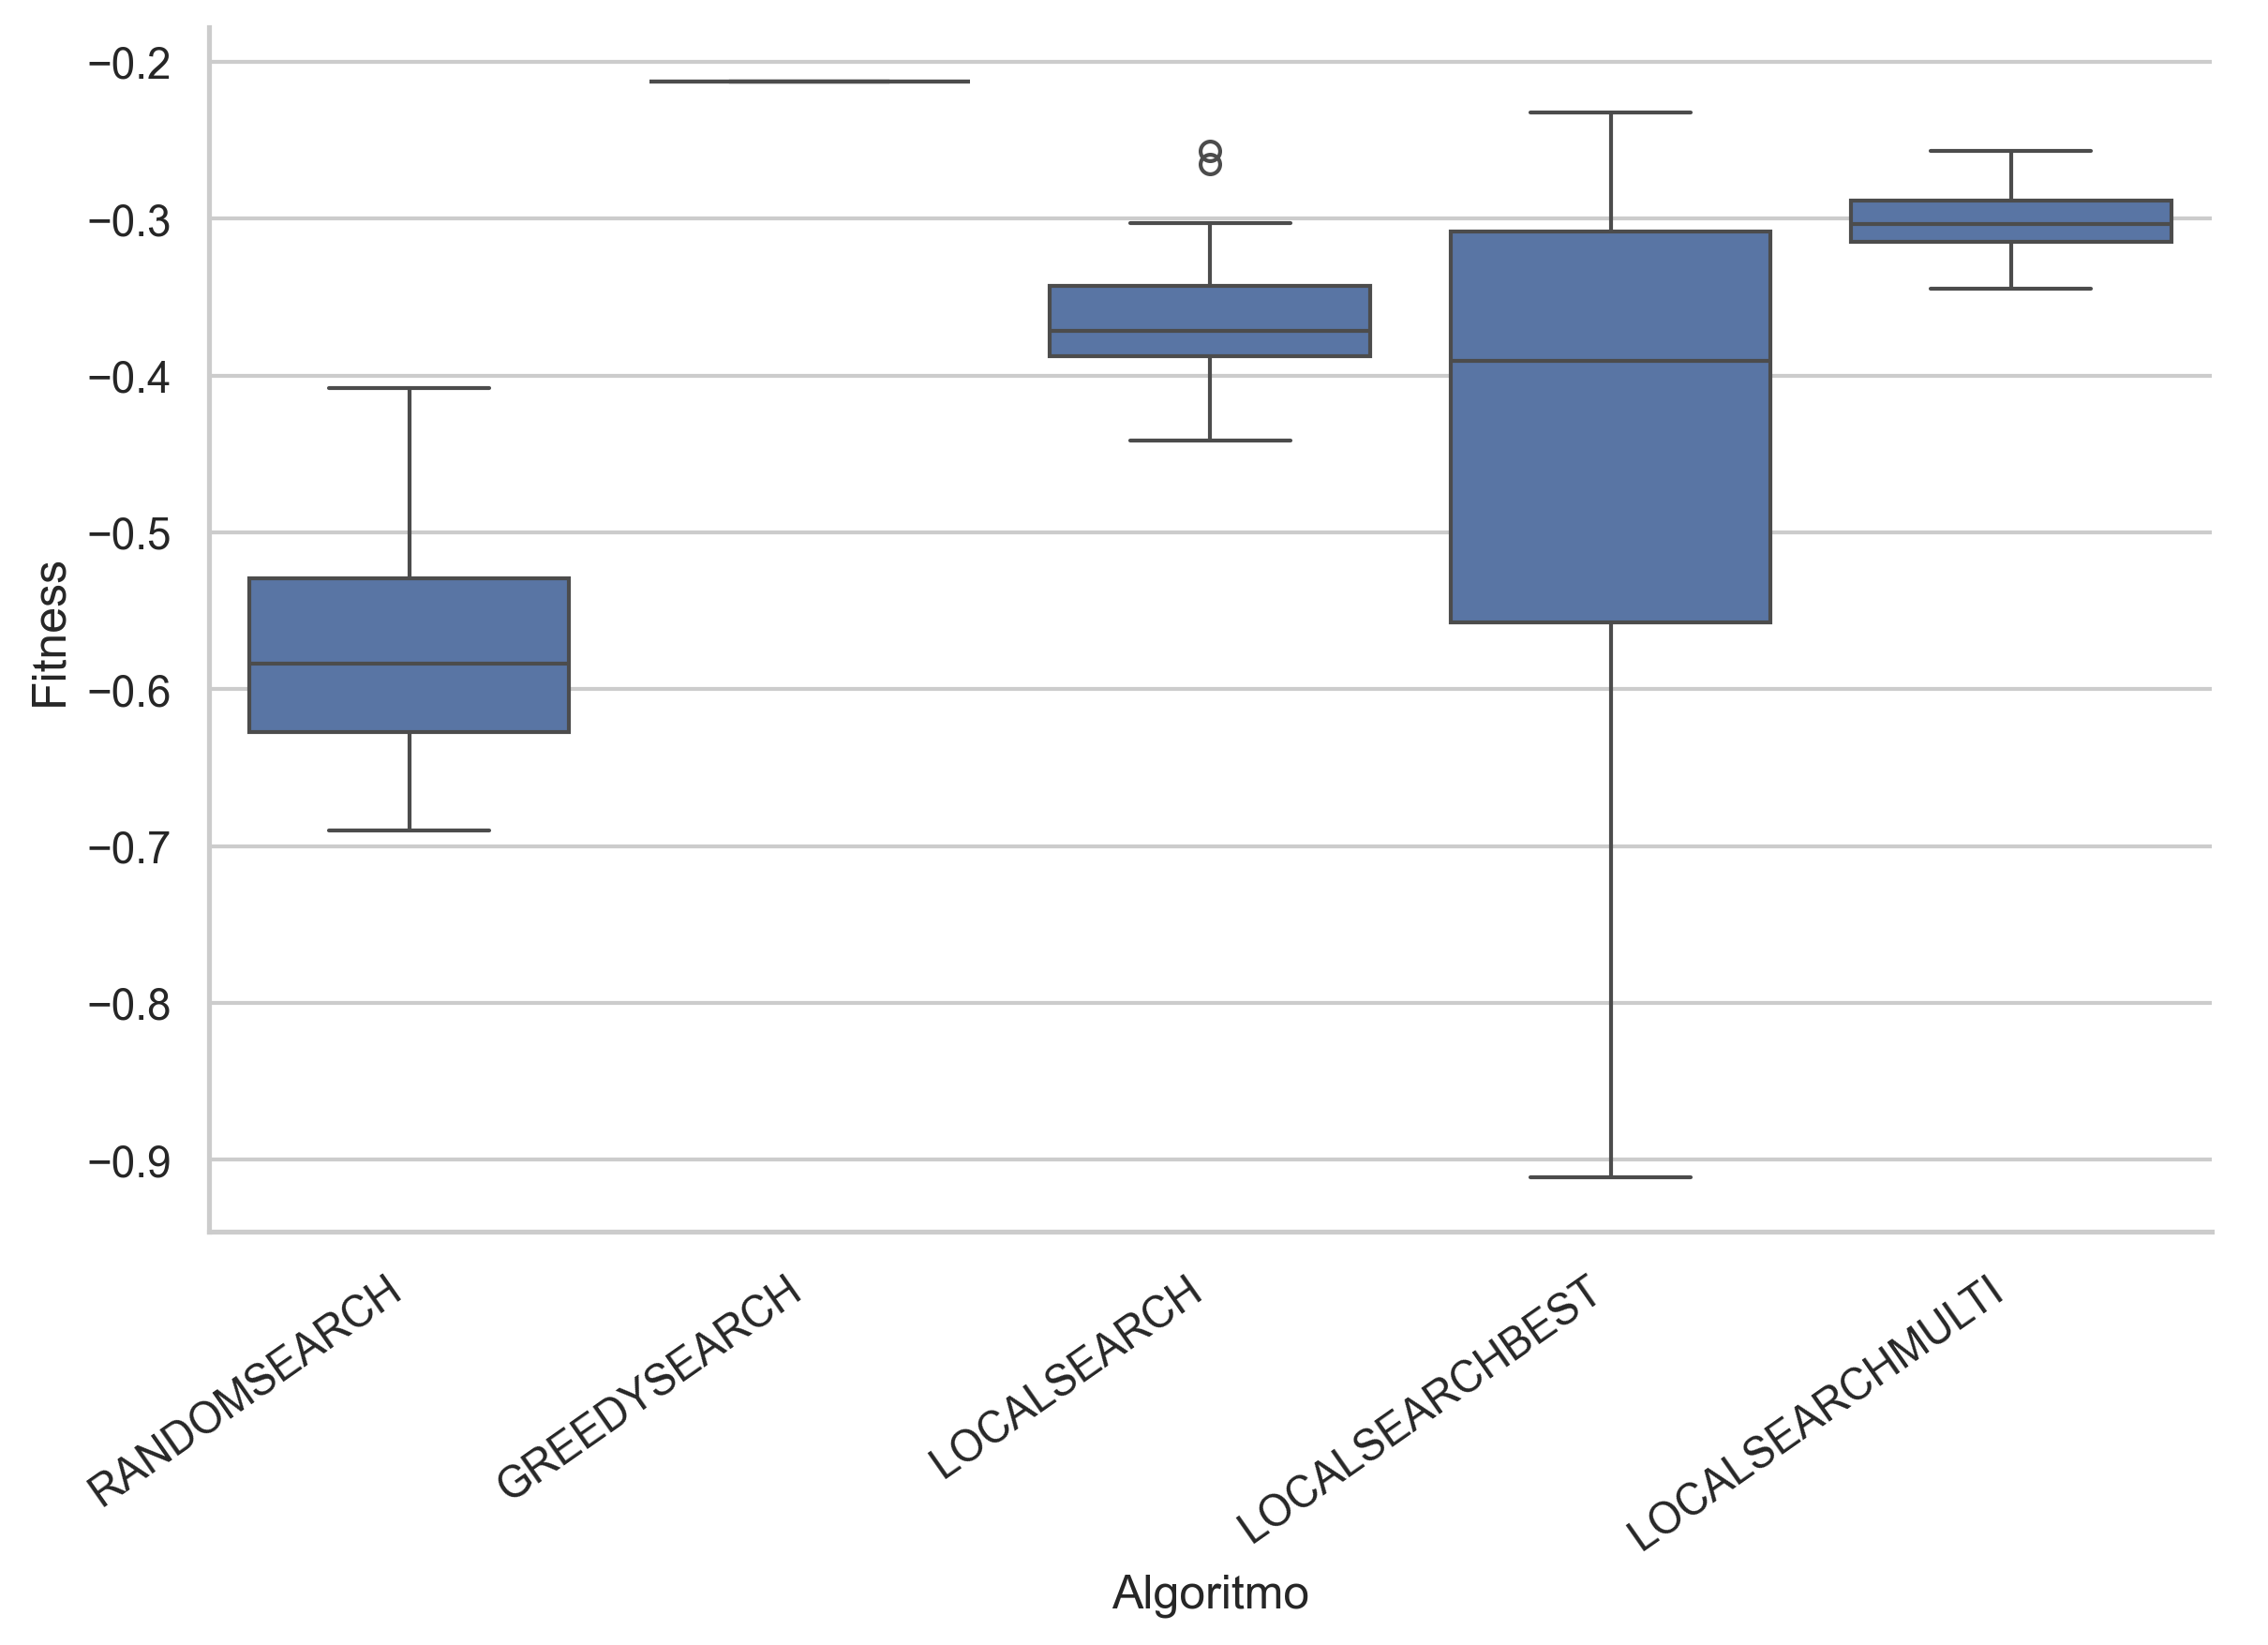
\includegraphics[width=0.65\textwidth]{figuras/IBEX_35_resultados.png}
    \caption{Distribución del Fitness por algoritmo en el mercado IBEX 35 ($N=30$)}
    \label{fig:ibex_box}
\end{figure}

\begin{figure}[htbp]
    \centering
    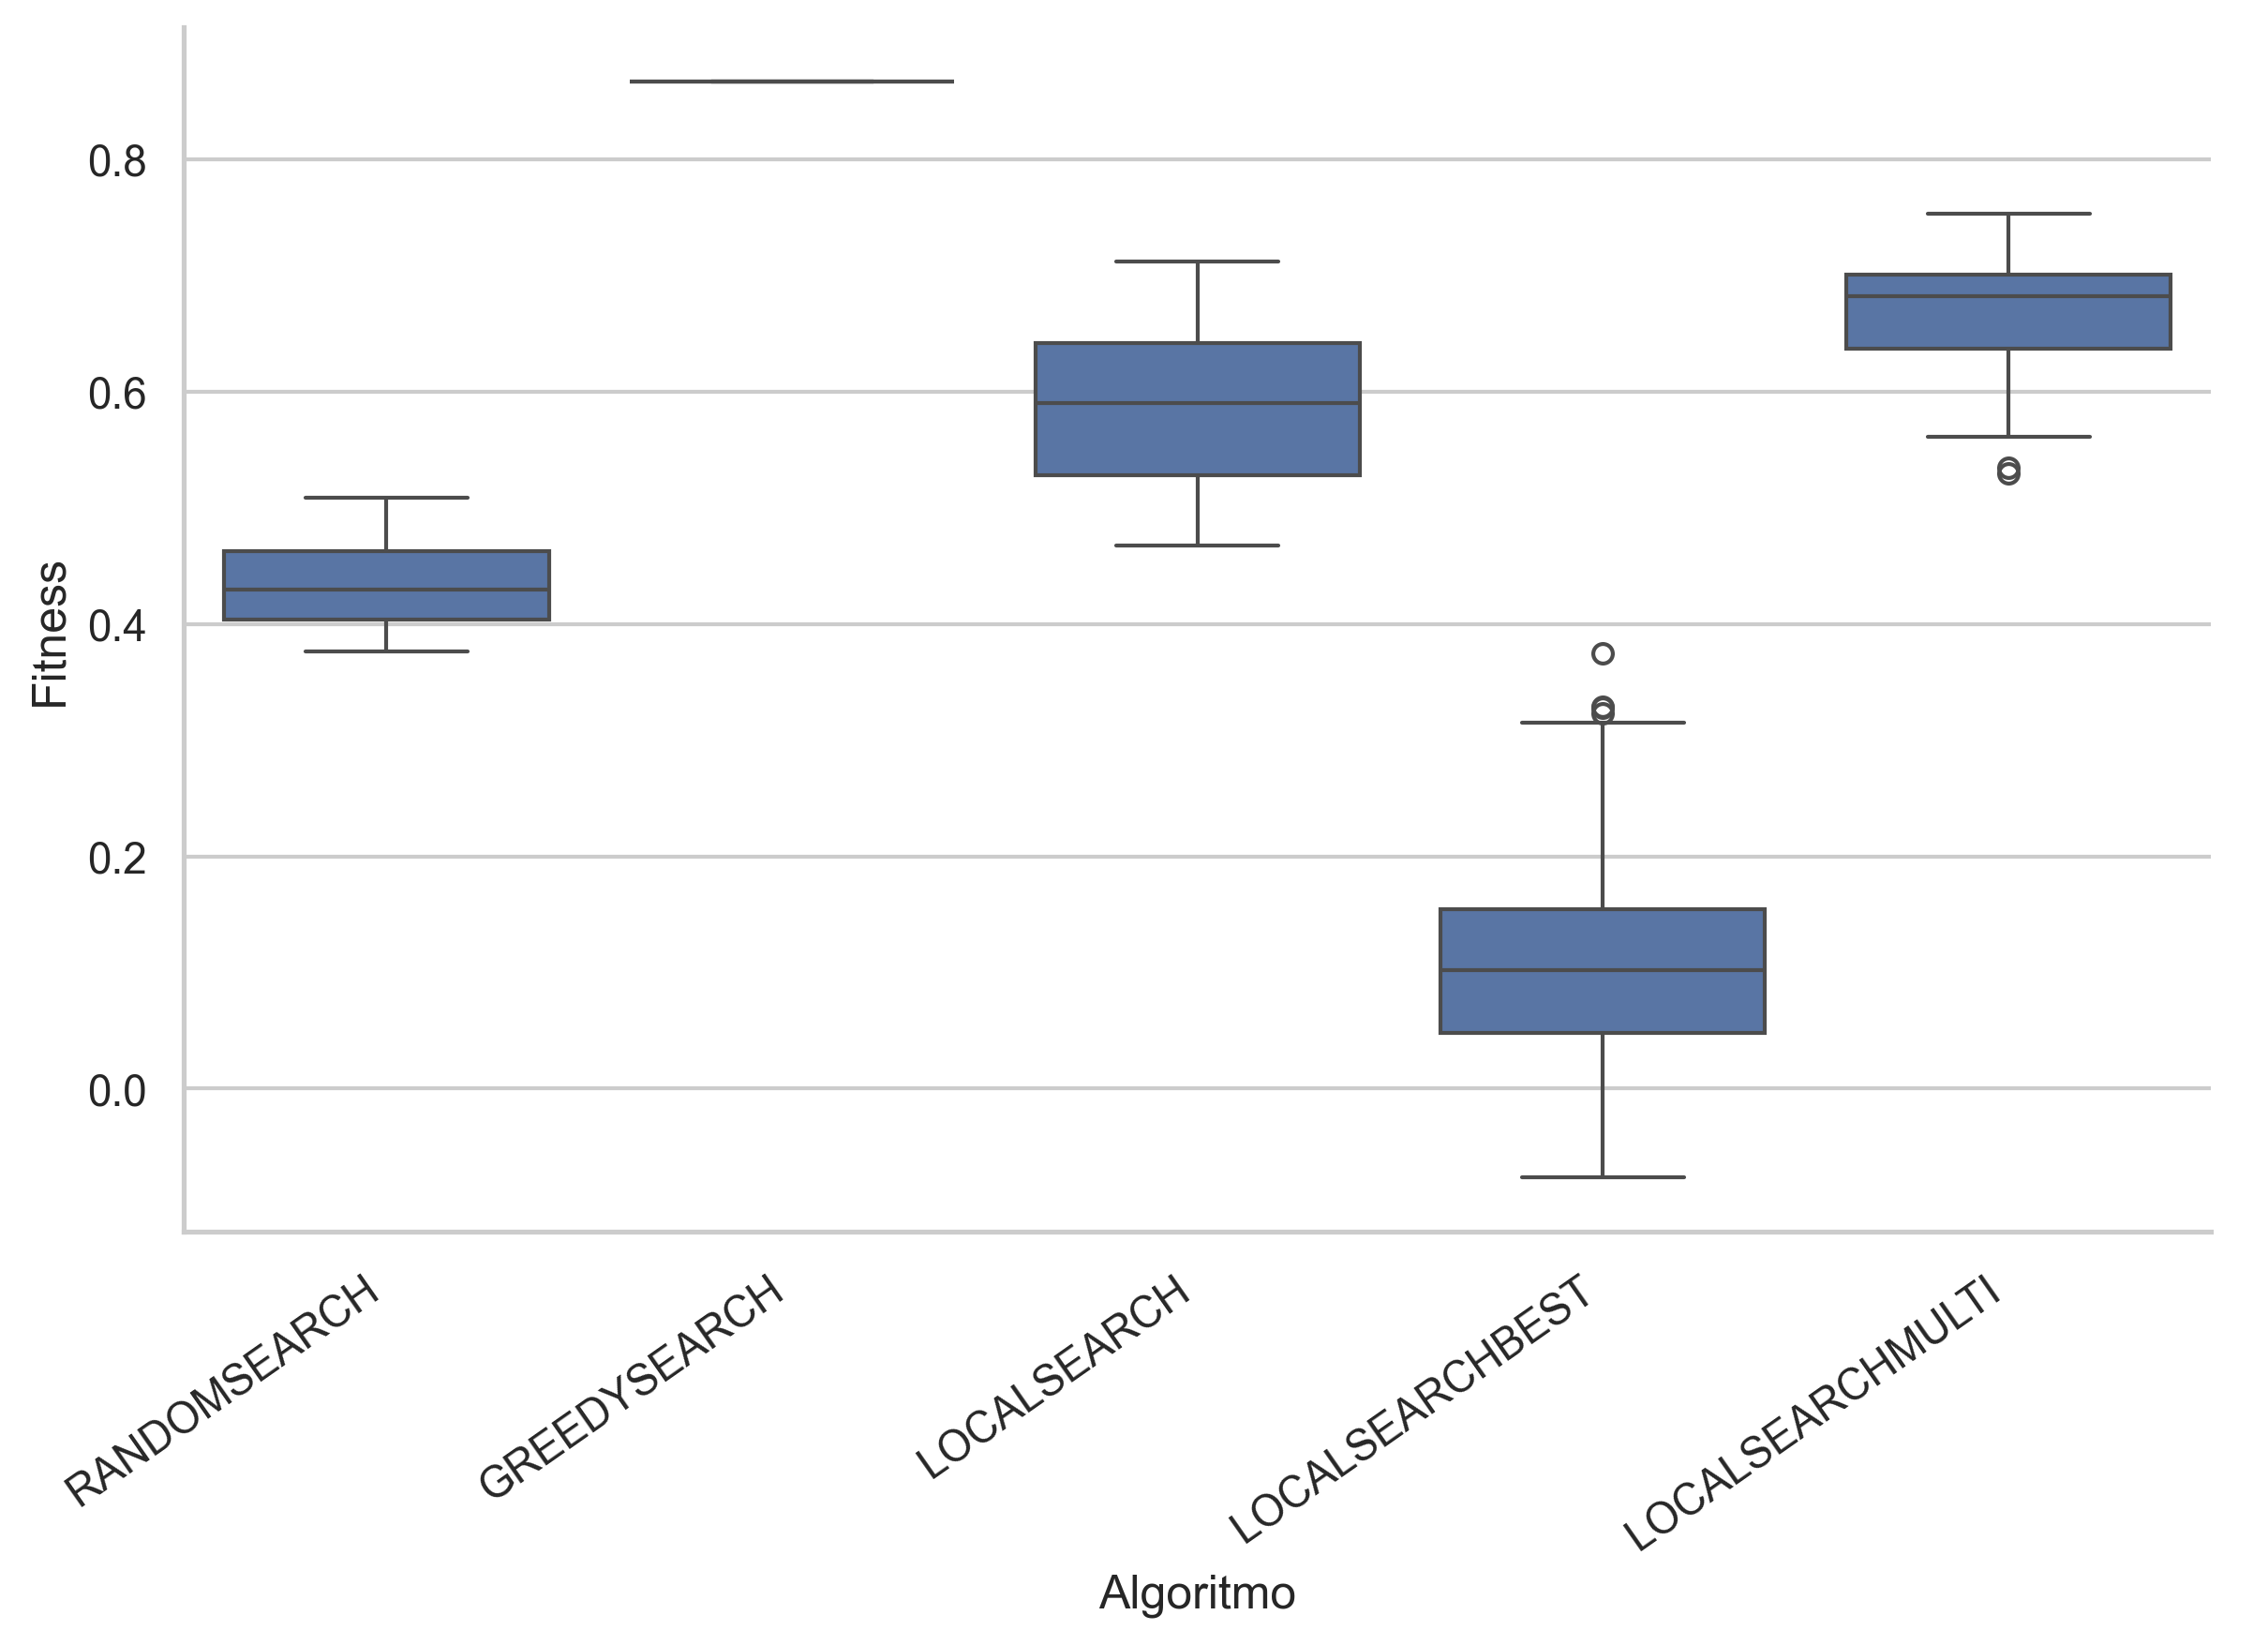
\includegraphics[width=0.65\textwidth]{figuras/S_P_100_resultados.png}
    \caption{Distribución del Fitness por algoritmo en el mercado S\&P 100 ($N=97$)}
    \label{fig:sp100_box}
\end{figure}

\begin{figure}[htbp]
    \centering
    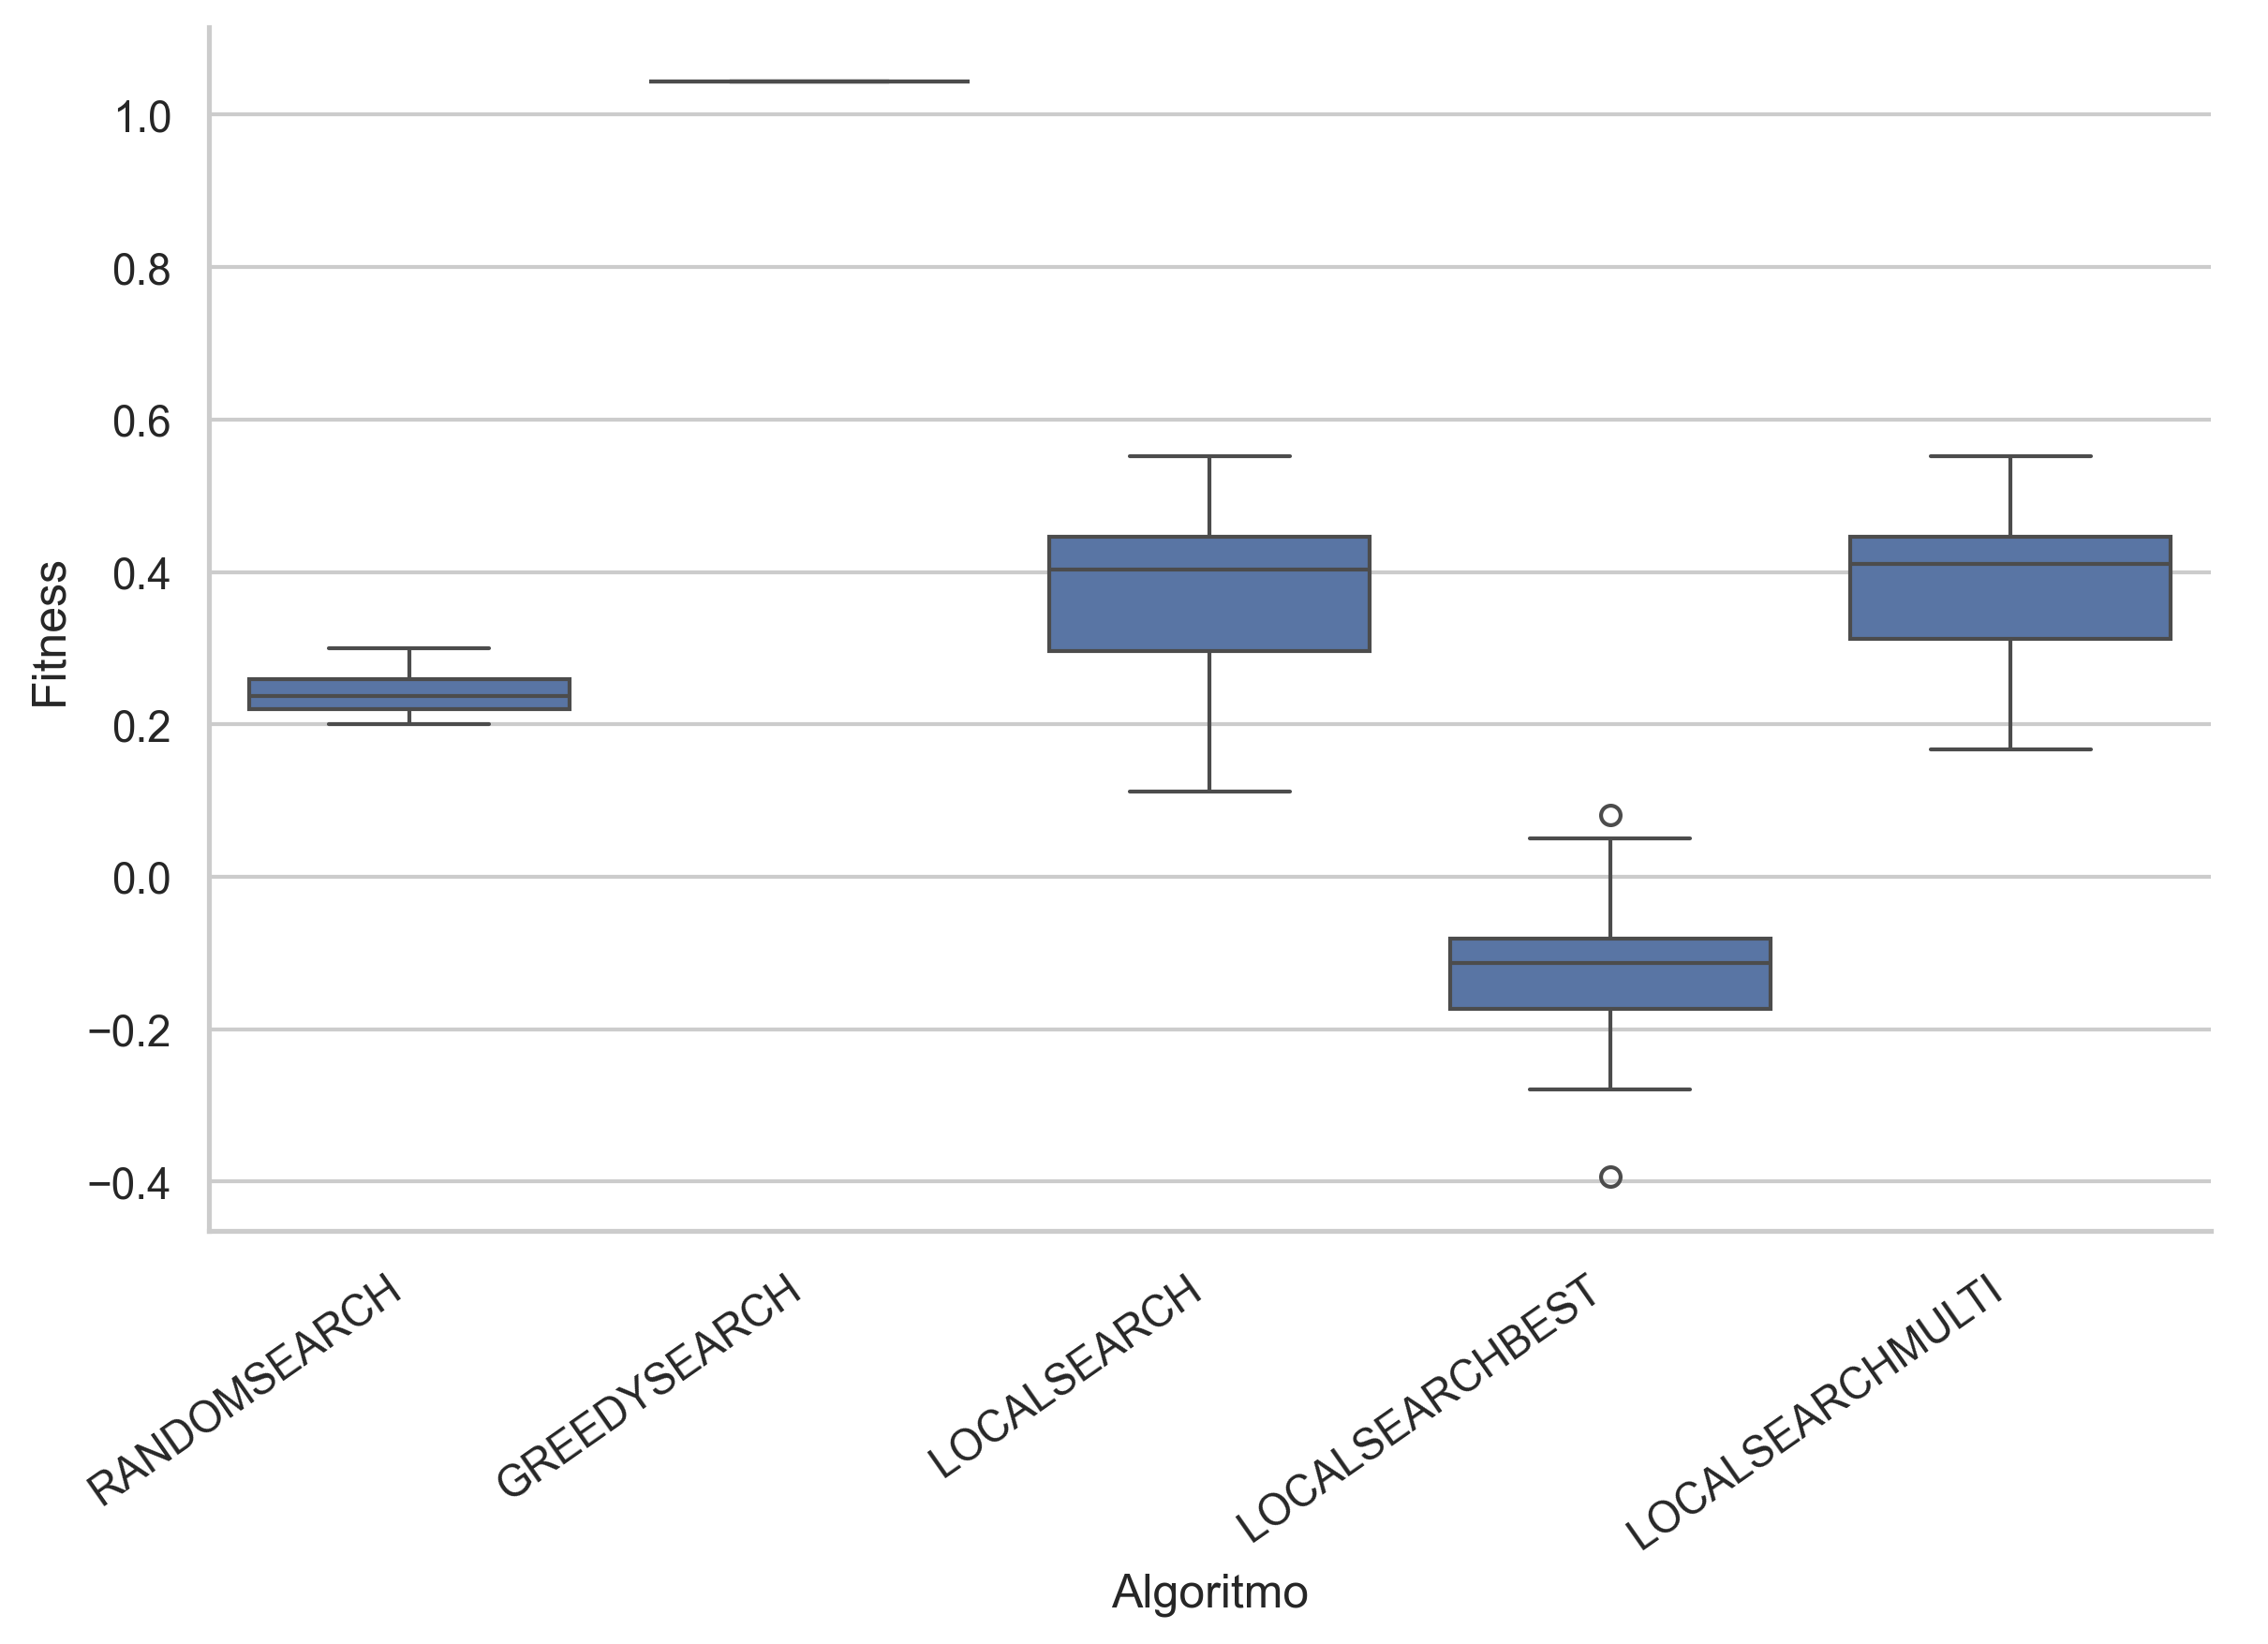
\includegraphics[width=0.65\textwidth]{figuras/S_P_500_resultados.png}
    \caption{Distribución del Fitness por algoritmo en el mercado S\&P 500 ($N=457$)}
    \label{fig:sp500_box}
\end{figure}

\subsection{Análisis Crítico de Resultados}
Al analizar conjuntamente los tiempos que tardan, cómo se comportan frente a los datos nuevos y lo que nos muestran los diagramas de caja, podemos sacar varias conclusiones interesantes sobre cómo encajan estos algoritmos con el modelo de Markowitz:

\begin{enumerate}
    \item \textbf{El engaño del algoritmo Greedy.}
    En los diagramas de caja, el \textit{Greedy Search} se visualiza como una línea plana en el extremo superior. Al carecer de componentes estocásticos, su varianza es nula, y logra el mejor \textit{fitness} histórico (ej. $1.043$ en S\&P 500). Sin embargo, las tablas revelan un colapso dramático en la validación (Test 2025): presenta el peor rendimiento real, con pérdidas del $-6.3\%$ en S\&P 500. Esto demuestra que la heurística voraz \textit{sobreajusta} ciegamente la cartera a los patrones del pasado, volviéndose extremadamente frágil ante variaciones futuras del mercado.

    \item \textbf{Mejorando poco a poco: óptimos locales en la Búsqueda Local.}
    Al comparar los métodos aleatorios, se nota enseguida que la Búsqueda Local (Local Search) rinde mucho mejor en entrenamiento que la Búsqueda Aleatoria (Random Search). Empezar desde una solución al azar e ir mejorando con el primer vecino bueno que encuentre ("First Improvement") hace que converja relativamente rápido (unas 875 evaluaciones de media en el IBEX 35). Sin embargo, nunca llega al nivel del Greedy en esta fase. Esto ocurre porque se suele quedar atascada en óptimos locales: la forma del espacio de búsqueda no le permite dar saltos lo suficientemente grandes como para probar configuraciones de pesos muy diferentes.

    \item \textbf{La Paradoja de la Aleatoriedad en la Generalización.}
    Paradójicamente, aunque la Búsqueda Aleatoria es la que peores resultados saca mirando al pasado (sus diagramas de caja son peores y muy dispersos), resulta ser la opción más prudente de cara al futuro. Por ejemplo, en el mercado S\&P 100, mientras el algoritmo Greedy nos hace perder dinero ($-4.1\%$), la Búsqueda Aleatoria nos da un beneficio de un $+6.4\%$. Al generar carteras más variables y evitar sobreoptimizar basándose en lo antiguo, ese "ruido" aleatorio nos sirve de escudo, diversificando la cartera de forma natural frente a la volatilidad que está por llegar.

    \item \textbf{Eficiencia Computacional y Escalabilidad.}
    A medida que los mercados son más grandes, el factor aleatorio empieza a pesar bastante más en el tiempo. En el S\&P 500 ($N=457$), la Búsqueda Local tarda menos ($1.540$ segundos) que la Búsqueda Aleatoria ($1.862$ segundos). La razón es sencilla: la Búsqueda Local solo necesita intercambiar un par de pesos para mutar el vector, evitando el altísimo coste temporal que tiene estar generando constantemente $457$ números aleatorios y arreglándolos a cada rato.
\end{enumerate}

\textbf{En conclusión:} El algoritmo Greedy es rapidísimo e imbatible cuando le preguntamos por el pasado, pero resulta peligroso para el futuro por su gran sobreajuste. La Búsqueda Local nos parece un mejor término medio: es más eficiente al no abusar de números aleatorios constantemente, y genera carteras mucho más estables. Aún así, nos deja claro que, si queremos evitar quedarnos estancados en los primeros óptimos locales que encuentre, tocará añadir algún mecanismo más inteligente para seguir explorando.